\documentclass[a4paper,10pt]{article}
%\documentclass[a4paper,10pt]{scrartcl}
\usepackage{pdfpages}
\usepackage[utf8]{inputenc}
\usepackage{ucs}
\usepackage{verbatim}
\usepackage{polski}
\usepackage[polish]{babel}
\usepackage{multicol}
% dodatkowe pakiety
\usepackage{enumerate}
\usepackage{hyperref} % references  as links
\usepackage{graphicx}
\DeclareGraphicsExtensions{.pdf,.png,.jpg}
\usepackage{epstopdf}
\usepackage{float}
\usepackage{color}
\usepackage{scalefnt}
\usepackage[square,sort,comma,numbers]{natbib}
\renewcommand{\contentsname}{Spis treści}
\renewcommand\bibname{Bibliografia}

\definecolor{mygreen}{rgb}{0,0.6,0}
\definecolor{mygray}{rgb}{0.5,0.5,0.5}
\definecolor{mymauve}{rgb}{0.58,0,0.82}
\usepackage{listings}
\lstset{ %
  texcl=true,
  backgroundcolor=\color{white},   % choose the background color; you must add \usepackage{color} or \usepackage{xcolor}
  basicstyle=\ttfamily\bfseries\footnotesize,       % the size of the fonts that are used for the code
  basewidth  = {.6em,0.6em},
  breakatwhitespace=false,         % sets if automatic breaks should only happen at whitespace
  breaklines=true, % sets automatic line breaking
  columns=fixed, 
  captionpos=t,                    % sets the caption-position to bottom
  commentstyle=\color{mygray},    % comment style
  deletekeywords={...},            % if you want to delete keywords from the given language
  escapeinside={\%*}{*)},          % if you want to add LaTeX within your code
  extendedchars=true,              % lets you use non-ASCII characters; for 8-bits encodings only, does not work with UTF-8
  frame=none,                    % adds a frame around the code
  keepspaces=true,                 % keeps spaces in text, useful for keeping indentation of code (possibly needs columns=flexible)
  keywordstyle=\color{blue},       % keyword style
  language=C++,                 % the language of the code
  morekeywords={*,...},            % if you want to add more keywords to the set
  numbers=left,                    % where to put the line-numbers; possible values are (none, left, right)
  numbersep=5pt,                   % how far the line-numbers are from the code
  numberstyle=\tiny\color{mygray}, % the style that is used for the line-numbers
  rulecolor=\color{black},         % if not set, the frame-color may be changed on line-breaks within not-black text (e.g. comments (green here))
  showspaces=false,                % show spaces everywhere adding particular underscores; it overrides 'showstringspaces'
  showstringspaces=false,          % underline spaces within strings only
  showtabs=false,                  % show tabs within strings adding particular underscores
  stepnumber=1,                    % the step between two line-numbers. If it's 1, each line will be numbered
  stringstyle=\color{mymauve},     % string literal style
  tabsize=4,                       % sets default tabsize to 2 spaces
  title=\lstname,
  inputencoding=utf8x,
  extendedchars=\true,% show the filename of files included with \lstinputlisting; also try caption instead of title
  literate={ą}{{\k{a}}}1
             {Ą}{{\k{A}}}1
             {ę}{{\k{e}}}1
             {Ę}{{\k{E}}}1
             {ó}{{\'o}}1
             {Ó}{{\'O}}1
             {ś}{{\'s}}1
             {Ś}{{\'S}}1
             {ł}{{\l{}}}1
             {Ł}{{\L{}}}1
             {ż}{{\.z}}1
             {Ż}{{\.Z}}1
             {ź}{{\'z}}1
             {Ź}{{\'Z}}1
             {ć}{{\'c}}1
             {Ć}{{\'C}}1
             {ń}{{\'n}}1
             {Ń}{{\'N}}1
}
\usepackage[fleqn]{amsmath}
\usepackage{mathtools}
\usepackage{latexsym}
\usepackage{pgfplots}
\pgfplotsset{compat=1.3}
\usepackage{pict2e}
\definecolor{blues6}{RGB}{198, 219, 239}
\definecolor{blues5}{RGB}{158, 202, 225}
\definecolor{blues4}{RGB}{107, 174, 214}
\definecolor{blues3}{RGB}{49, 130, 189}
\definecolor{blues2}{RGB}{8, 81, 156}
\definecolor{blues1}{RGB}{1, 1, 1}

\pgfplotscreateplotcyclelist{colorbrewer-blues}{
{blues1},
{blues2},
{blues3},
{blues4},
{blues5},
{blues6},
}


\title{Sieci neuronowe $\spadesuit$}
\author{Piotr Grabowski $\clubsuit$ $\clubsuit$}
\date{\today}

\pdfinfo{%
  /Title    ()
  /Author   ()
  /Creator  ()
  /Producer ()
  /Subject  ()
  /Keywords ()
}
\usepackage{graphicx}
%\usepackage{graphics}
\input{epsfx}
\usepackage{epsfig}
\usepackage{url}
\usepackage[utf8]{inputenc}
\usepackage[T1]{fontenc}
\usepackage[polish]{babel}
\usepackage{geometry}
\usepackage{ulem}
\usepackage{lipsum}
\usepackage{listings}
\usepackage{url}
\usepackage{color}
\usepackage{xcolor}
\selectlanguage{polish}
\usepackage{hyperref}
\begin{document}
\maketitle

\url{http://iisi.pcz.pl/nn/podstawy.php} 

\tableofcontents
\section{Wykład 1 - wprowadzenie $\heartsuit$ }

\paragraph{Podstawowe cechy sieci neuronowych}

\begin{enumerate}
 \item adaptacja i samoorganizacja
 \item zmniejszona wrażliwość na uszkodzenia elementów
 \item równoległa praca
 \item wygoda programowania przez uczenie
\end{enumerate}

\paragraph{Zastosowania}

\begin{enumerate}
 \item klasyfikacja obrazów
 \item klasteryzacja / kategoryzacja
 \item aproksymacja funkcji 
 \item predykcja / prognozowanie
 \item optymalizacja
 \item odtwarzanie
 \item sterowanie
\end{enumerate}

\paragraph{Przepływ sygnału w NN}

\begin{enumerate}
 \item warstwa wejściowa
 \item warstwa ukryta
 \item warstwa wyjściowa
\end{enumerate}

Warstwa wejściowa nie może się uczyć. (jak jest warstwa wejściowa, 2 ukryte i wyjściowa to jest 
to sieć trójwarstwowa (wejściowa się nie liczy))

W warstwie ukrytej są neurony ukryte. Mogą być nieliniowe. Warstwa wyjściowa nie różni się niczym
od ukrytej poza tym, że jest jedna i wyjścia z niej są wyjściami z sieci.
\section{Wykład 2 - wstęp do neurofizjologii $\heartsuit$ $\heartsuit$}

Mózg waga $1250 - 1400\ g$, $100$ mld neuronów, dzienny ubytek $10$ tyś., liczba połączeń $100$ tyś mld,
szerokość synaps ($20-25$ nanometrów - szerokość $\frac{1}{600}$ włosa. Zużycie glukozy $20\%$ większe
niż inne narządy, zużycie tlenu $20\%$, intensywność ukrwienia $750$ ml/min, energii $10$ WAT.

Neuron składa się z dendrytów , jądra komórki (na niej ziarnistości - soma) i aksonu. (na koniec kolaterale końcowe)
Wejścia presynaptyczne (akson) do jądra (neuronu postsynaptycznego).

\paragraph{Rodzaje neuronu}

\begin{enumerate}
 \item jednobiegunowy, dwubiegunowy, gwiaździsty
 \item purkinjego, kłębuszkowy, golgiego
\end{enumerate}

Na końcu aksonu jest synapsa (kolbka synaptyczna). Dotyka ciała komórki odbiorczej. Synapsa składa
się z neurogibryli , mitochondrium, aparatu Golgiego, pęcherzyków synaptycznych i błony pre i post synaptycznej.

Typowy kierunek przemieszczania się sygnału jest od dentrytu do aksonu, ale może następować odwrotny przepływ sygnału.
pojedyncze neurony mogą wysyłać sygnały nawet przy braku
elektrycznej stymulacji w obrębie ciała komórki czy dendrytów.
Procesy pamięciowe komórek zachodzą w aksonach, a potencjał iglicowy jest generowany dalej (bliżej końca aksonu).
Aksony komunikują się ze sobą. 

\paragraph{Schemat funkcjonowania synapsy}

\begin{enumerate}
 \item neurotransmiter
 \item pęcherzyk synaptycznych
 \item enzym rozkładający
 \item receptor presynaptyczny
 \item receptor postsynaptyczny
\end{enumerate}

\paragraph{Neurotransmitery}

\begin{enumerate}
 \item serotonina
 \item acetylocholina
 \item adrenalina
 \item dopamina
\end{enumerate}

\paragraph{Polaryzacja błony komórkowej}

\begin{enumerate}
 \item potencjał spoczynkowy -70mV
 \item potencjał czynnościowy -59mV (od synapsy pobudzającej)
 \item hiperpolaryzacja (od synapsy hamującej) -80mV
\end{enumerate}

Istnieje mechanizm sygnalizacji wstecznej - endokanabinoidy działają wstecz, przemieszczają się
z neuronu postsynaptycznego do presynaptycznego. Hamuje wytwarzanie się neuroprzekaźnika GABA.

\paragraph{Model neuronu McCullocha-Pittsa 1943}

\begin{equation}
  y^{k+1}= 
\begin{cases}
    1,& \text{if } \sum_{i=1}^n w_i x_i^k \ge T \\
    0,              & \text{otherwise}
\end{cases}
\end{equation}

$x_i^k$ - sygnały wejściowe, mówią, czy w chwili $k$ pojawił się sygnał czy nie, $y$ - wyjście neuronu.
$w_i$ może być dodatni (synapsa pobudzająca) i ujemny (hamująca), $T$ jest wartością progową.

\paragraph{Wierny model pojedynczego neuronu}

32000 równań różniczkowych, 19200 parametrów do oszacowania.

\begin{figure}[H]
 \centering
 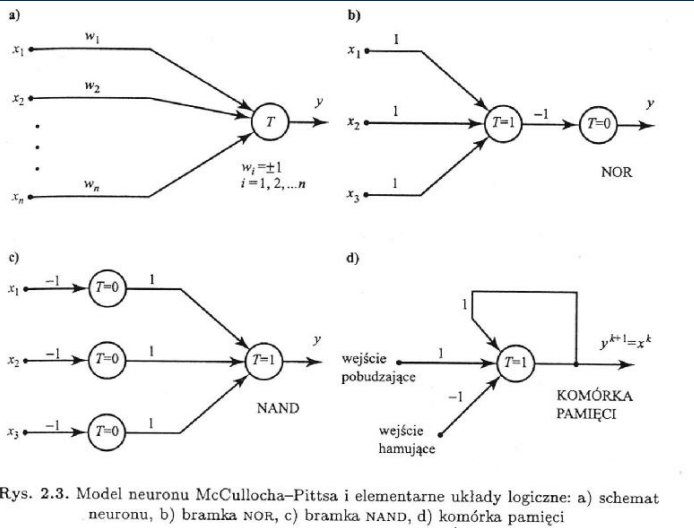
\includegraphics[scale=0.6]{sieci1}
\end{figure}
\section{Wykład 3 - liniowe i nieliniowe sieci neuronowe $\heartsuit$ $\heartsuit$ $\heartsuit$  }

\begin{enumerate}
 \item jądro - centrum obliczeniowe neuronu, to są kluczowe procesy
 \item akson - wyjście neuronu, ma tylko jedno wyjście
 \item wzgórek aksonu - sumowanie przychodzących sygnałów i generowanie potencjałów czynnościowych, które
 wędrują przez akson
 \item dendryt - wejście neuronu, może być wiele, biologiczne neurony mają ich tysiące
 \item synapsa - jeśli dendryt jest wejsciem neuronu to synapsa jest furtką. ma wpływ na moc sygnału napływającego poprzez akson.
\end{enumerate}

\paragraph{Ogólna definicja neuronu}

\begin{equation}
 y = f(\phi(x_i w_i))
\end{equation}

\begin{enumerate}
 \item $\phi$ - Post synaptic potential (potencjał postsynaptyczny)
 \item $f$ - funkcja aktywacji
 \item $x_i$ - wejścia
 \item $w_i$ - wagi
 \item $y$ - wyjście
\end{enumerate}

\paragraph{Definicja neuronu}

\begin{equation}
 y = f(\sum(x_i w_i))
\end{equation}

Zamiast PSP blok sumujący.

\paragraph{Neuron liniowy}

\begin{equation}
 y = \sum(x_i w_i)
\end{equation}

Brak funkcji aktywacji.

\paragraph{Neuron z funkcją skokową (nieliniowy neuronik)}

$f(x)$ jest takie, że jeśli $x$ jest większe od progu to robi skok (podaje $1$), inaczej $0$.

\paragraph{BIAS (przesunięcie) oraz PRÓG (threshold)}

\begin{equation}
 e = b + \sum_{i=1}^n x_i w_i
\end{equation}

Można przyjąć, że $w_0 = b$ i wtedy bias jest jak każda inna waga, z tym, że sygnał $x_0$ jest równy $1$.
Wtedy:
\begin{equation}
 e = \sum_{i=0}^n x_i w_i
\end{equation}

Funkcję aktywacji można wtedy przyjąć jako:

\begin{equation}
  f(e)= 
\begin{cases}
    1,& \text{if } e \ge 0 \\
    0,              & \text{otherwise}
\end{cases}
\end{equation}

Możemy uznać, że bias jest stałym progiem wtedy:

\begin{equation}
 e = \sum_{i=1}^n x_i w_i
\end{equation}

oraz

\begin{equation}
  f(e)= 
\begin{cases}
    1,& \text{if } e \ge \theta \\
    0,              & \text{otherwise}
\end{cases}
\end{equation}

gdzie $\theta$ to próg.

Pierwszy wniosek jest taki, że $\sum x_i w_i$ jest prostą, płaszczyzną, i hiperpłaszczyzną (zależy od wymiaru).

Druga różnica jest taka, że przy założeniu, że $w_2$ jest różne od $0$ wzory na granicę pomiędzy $0$, a $1$ na wyjściu są takie:
(dla 2 wymiarów)
\begin{equation}
 x_2 = - \frac{w_1}{w_2} - \frac{b}{w_2}
\end{equation}

oraz

\begin{equation}
 x_2 = - \frac{w_1}{w_2} + \frac{\theta}{w_2}
\end{equation}

Jak jest próg stały to uwaga... podczas nauki się nie zmienia! A jak nie jest stały to uwaga.. się zmienia!
I to czy ma być stały czy nie zależy od problemu. Bo raz zadziała, raz nie... heheszki.

Dyskryminacja liniowa - wykres przedstawiający linię oddzielającą $0$ od $1$ dla różnych $x$
(np. w 2d)

Powierzchnia odpowiedzi - dodajemy 3 wykres - wartość wyjścia - dyskryminacja liniowa jest rzutem na powierzchnię odpowiedzi od góry na iksy

\paragraph{Neuron liniowy - screeny od Tadka}

Wejścia i wyjścia w neuronie mogą być znormalizowane (patrz Tadeusiewicz, ale lepiej nie) od $-1$ do $1$.

I można zapisać wzory wektorowo:
\begin{equation}
 y = W^T X
\end{equation}

co jest najzwyczajniejszym na świecie mnożeniem iksy przez wartości. Jednak jeśli $x_i$ i $w_i$ są
znormalizowane to 
\begin{equation}
 y = cos \phi
\end{equation}

gdzie $\phi$ jest kątem pomiędzy wektorami $W$ oraz $X$. Prosty wniosek, że sygnał będzie tym większy
im bardziej kąt będzie mniejszy (czyli wektory będą skierowane bardziej w tą samą stronę).

Można też zapisać to macierzowo.

W sieci liniowej nie robi się warstw ukrytych z zasady, bo nie wzbogacą zachowania sieci.
(algebra)

\paragraph{ADALINE - Adaptive Linear Element - Reguła Widrow-Hoffa}

Regułę robimy następująco:
\begin{equation}
 W' = W + \mu \delta X
\end{equation}

albo za pomocą wzoru 

\begin{equation}
 W' = Z X^{-1}
\end{equation}

$mu \ge 0$. Jak $\delta = z - y$ jest $\ge 0$ to znaczy, że $z > y$ czyli odpowiedź sieci była za mała.
A jak $\delta < 0 $ to $ z < y $ czyli odpowiedź była za duża.

Jak odpowiedź była za mała to $W'$ się zwiększa, jak za duża to $W'$ się zmniejsza.

Można udowodnić, że reguła ta optymalizuje wagi względem funkcji celu:
\begin{equation}
 Q = \frac{1}{2} \sum_{i=1}^N {(z^j - y^j)}^2
\end{equation}
za pomocą poszukiwania minimum metodą gradientową.

MADALINE to jest Wiele ADALINE i Reguła Widrow-Hoffa również działa.
\section{Wykład 4 - Sieci Kohonena uczenie bez nauczyciela $\heartsuit$ $\heartsuit$ $\heartsuit$ $\heartsuit$}

\paragraph{Reguła Hebba}

\begin{equation}
 W' = W + n y X
\end{equation}

Analogiczna do Widrow-Hoffa, ale zamiast błędu mamy po prostu sygnał wyjściowy.

Wady Hebba:

\begin{enumerate}
 \item niska efektywność uczenia
 \item przemnożony wpływ początkowych wart. wag
 \item możliwość pomijania niektórych klas nauczonej sieci
 \item powstawanie reduntantnych nadinterpretacji klas
\end{enumerate}

Uczenia polega na tym, że wektory id do sygnału wejściowego uczącego.
Zasada owczego pędu - idą wszystkie. Może być za duży albo za mały współczynnik uczenia.
Czas nauki jest istotny. Bardzo duża liczba neuronów może nie pomagać. Sieć może zapomnieć 
klasy (wektory zostały \textit{ukradzione})

\paragraph{Warianty metod samouczenia}

Metoda przyrostowego samouczenia (differential hebbian learning)

\begin{equation}
 w_{ki}^{j+1} = w_{ki}^j + \mu (x_i^j - x_i^(j-1))(y_k^j - y_k^(j-1))
\end{equation}

Metoda \textit{Gwiazdy wejść} (Instar learning) - najczęściej wybierana w analizie skupień

\begin{equation}
 w_{ki}^{j+1} = w_{ki}^j + \mu^j (x_i^j - w_{ki}^j)
\end{equation}
\begin{equation}
 \mu^j = 0.1 - \lambda
\end{equation}

Miarą podobieństwa wektora wejściowego i wektora wag jest cosinus kąta unormowanych wektorów.

Metoda \textit{Gwiazd wyjść} (Outstar learning)

\begin{equation}
 w_{ki}^{j+1} = w_{ki}^j + \mu^j (y_k^j - w_{ki}^j)
\end{equation}

\paragraph{Samouczenie sieci metodą Kohonena}

Po pojawieniu się sygnału wejściowego wszystkie sygnały wyjściowe są porównywane i wybierany jest
\textbf{zwycięzca} o numerze $k$, którego sygnał $y_k^j$ ma \textbf{największą} wartość. Wówczas
zmieniamy współczynnik w następujący sposób:

\begin{equation}
 w_{ki}^{j+1} = w_{ki}^j + \mu (x_i^j - w_{ki}^j)
\end{equation}

Można zdefiniować pojęcie sąsiedztwa:

\begin{equation}
 w_{mi}^{j+1} = w_{mi}^j + \mu h(m,k) (x_i^j - w_{mi}^j)
\end{equation}

funkcja $h(m,k)$ jest malejącą funkcją odległości między neuronem $m$, a zwycięzcą $k$.

Zasady rywalizacji:
\begin{enumerate}
 \item ZWYCIĘZCA BIERZE WSZYSTKO ( WINNER TAKES ALL)
 \item ZWYCIĘZCA BIERZE WIĘKSZOŚĆ ( WINNER TAKES MOST)
\end{enumerate}

Mapa topologiczna w korze mózgowej w obszarze czucia somatycznego oraz sterowania jest o podobnej 
strukturze, co sieci Kohonena.
Istnieje zjawisko skręcenia się sieci Kohonena np. w postać krzyża.
SOM może być wykorzystywana do przedstawiania skomplikowanych korelacji w danych statystycznych.
Sieć Kohonena może służyć do rzutowania wielowymiarowego zbioru danych do przestrzeni o małej wymiarowości.

\paragraph{Mechanizm sumienia}

Istnieje możliwość wprowadzenia sumienia, wtedy niwelujemy możliwość dłuższego braku nauki jakiegoś neuronu.

\paragraph{Podsumowanie}

\begin{enumerate}
 \item sieć uczy się bez nauczyciela
 \item ma dwie warstwy o wyraźnie rozdzielonych funkcjach (wejściowa i topologiczna)
 \item uporządkowane neurony wyjściowe
 \item ważną rolę odgrywa sąsiedztwo
 \item w wyniku uczenia powstaje mapa topologiczna
 \item apriorytyczna interpretacja wartości wyjściowych jest niemożliwa
 \item po uczeniu można ustalić jakie znaczenie mają poszczególne rejony mapy topologicznej - ale 
 tylko na podstawie analizy konkretnych danych wejściowych
\end{enumerate}

\paragraph{Zastosowania}

\begin{enumerate}
 \item rozpoznawanie obrazów
 \item klasyfikacja
 \item zgłębianie danych
 \item tworzenie modeli - modelu świata zewnętrznego w mózgu robota, modelu uczciwego przedsiębiorcy albo działania procesu
\end{enumerate}
\section{Wykład 5 - sieci CP i LVQ $\heartsuit$ $\heartsuit$ $\heartsuit$ $\heartsuit$ $\heartsuit$}

\paragraph{Uczenie z forsowaniem}

\begin{equation}
 w_{ki}^(j+1) = w_{ik}^j + \mu z_k^j x_i^j
\end{equation}

Maksymalna liczba możliwych do zapamiętania wzorów w sieci o k neuronach
\begin{equation}
 N_{max} = \frac{k}{2 log{k}}
\end{equation}

Efekty uczenia (przy założeniu, że wszystkie wektory wejściowe są ortonormalne) sieć:
\begin{enumerate}
 \item uczy się wiernie odtwarzać wymagane reakcje na wszystkie rozważane sygnały wejściowe
 \item potrafi uśredniać wejściowe sygnały i odtwarzać idealny wzorzec serii przypadkowo zniekształconych
 obserwacji
\end{enumerate}

\paragraph{Architektura sieci LVQ}

Sieć składa się z warstwy wyjściowej, warstwy kohonena oraz warstwy wejściowej. 

Sieć LVQ służy do klasyfikacji sygnałów wejściowych i jest przykładem uczenia z forsowaniem. 
Warstwa wyjściowa przypisuje wektory wyjściowej do jednej z kilku klas. Główną częścią sieci jest
warstwa kohonena dokonująca klasyfikacji. LVQ daje \textbf{jednakową liczbę neuronów} przypisanych do danej klasyfikacji

Podklasy w danej grupie nie muszą być podobne.

Podczas uczenia obliczana jest odległość wektora wejściowego od wszystkich neuronów warstwy i wyłaniany 
jest najbliższy zwycięzca. Jeśli wygrywający wektor należy do klasy sygnału, który pojawił się na wejściu
to jego wagi są modyfikowane tak, aby zbliżyć się do prezentowanego sygnału. Jeśli nie należy to wektor 
ten jest odsywany co jest określane jako \textit{odpychanie}. Podczas procesu uczenia neuron 
przypisany do danej klasy wędruje do obszaru związanego z tą kategorią.
W trybie testowania (klasyfikacji) obliczana jest odległość prezentowanego neuronu wejściowego 
do każdego neuronu i leżący najbliżej zostaje zwycięzca. Przynależność do klasy tego sygnału wskazuje
ten zwycięski neuron.

\begin{equation}
 d_i = || w_i - x || = \sqrt{ \sum_{j=1}^N (w_{ij} - x_j)^2 }
\end{equation}

\paragraph{Modyfikacja wag zwycięskiego neuronu}

\begin{equation}
 W' = \begin{cases}
    w + \alpha (x-w),& \text{if neuron należy do właściwej klasy} \\
    w - \gamma (x-w) & \text{otherwise} 
\end{cases}
\end{equation}



\paragraph{Wariant LVQ \#1}

Istnieje możliwość wprowadzenia pojęcia \textit{sumienia}. Jeśli neuron wygrywa zbyt często oddaje
je innemu neuronowi. Realizowane jest to poprzez bias:
\begin{equation}
 d_i' = d_i + b_i
\end{equation}

\begin{equation}
 d_i = ||w_i - x|| = {\left(\sum_{j=1}^N (w_{ij} - x_j)^2 \right)}^2
\end{equation}

\begin{equation}
 b_i = \mu d_{i_{max}} (1 - N p_i)
\end{equation}

\begin{enumerate}
 \item $d_{i_{max}}$ największa odległość wyestymowana wewnętrznie (?)
 \item $\mu$ - stała, która zwalnia proces uczenia
 \item $p_i$ oblicza częstotliwość wygrywania, na początku $\frac{1}{N}$
 \item liczba neuronów kohonena na klasę
 \item $\phi$ stała do aktualizacji częstotliwości wygrywania
\end{enumerate}

\begin{equation}
 W' = \begin{cases}
    (1-\phi) p_i,& \text{if i nie jest zwycięzcą w klasie} \\
    (1 - \phi) p_i + \phi, & \text{otherwise}
\end{cases}
\end{equation}

Wybiera się globalnego zwycięzce obliczając odległość $d_i$ i lokalnego zwycięzce, ale z tej klasy
biorąc pod uwagę $d_i'$. Wagi lokalnego zwycięzcy są modyfikowane w następujący sposób:

\begin{equation}
 W' = \begin{cases}
    w + \alpha (x-w),& \text{if neuron jest globalnym i lokalnym zwycięzcą} \\
    w - \beta (x-w) & \text{otherwise} 
\end{cases}
\end{equation}

podczas, gdy globalny zwycięzca jest odrzucany od wektora wejściowego zgodnie ze wzorem:

\begin{equation}
 w' = w - \gamma (x - w)
\end{equation}
jeśli globalny zwycięzca nie jest we właściwej klasie

\paragraph{Wariant LVQ \#2}

Jeśli w sieci jest neuron zwycięzca z wektorem wag $w_1$, który nie wskazuje na klasę sygnału
wejściowego, a drugi następny w kolejności o wagach $w_2$ właśnie z tej klasy to w takiej wersji
LVQ zwycięzca jest odpychany od sygnału wejściowego, drugi natomiast jest traktowany jak zwycięzca 
pod warunkiem, że odległość wektora wejściowego od obu wybranych neuronów jest podobna

\begin{equation}
 w_1 = w_1 - \alpha (x - w)
\end{equation}

\begin{equation}
 w_2 = w_2 - \alpha (x - w)
\end{equation}

\paragraph{Strategia uczenia sieci LVQ}

Podstawowy proces uczenia sieci LVQ polega na obliczeniu odległości w sensie metryki euklidesowskiej
pomiędzy wektorami $w_i$ (wektor wagi), a wektorem $x$ (norma średniokwadratowa):

\paragraph{Sieci Counter Propagation}

zaproponowane przez Robarta Hecht-Nielsens, kompilacja sieci Kohonena i Grosberga, szybciej się uczą (w przeciwieństwie
do sieci ze wsteczną propagacją). Przy pomocy CP można szybko weryfikować hipotezy robocze

\begin{equation}
 || x || = 1
\end{equation}

Normalizacja wektorów wejściowych
\begin{equation}
 x_i' = \frac{x_i}{ \sqrt{ \sum_{j=1}^n x_j^2 }  }
\end{equation}

Pierwsza warstwa realizuje algorytm Kohonena:

\begin{equation}
 e_j = W_j^T X
\end{equation}

\begin{equation}
 k_j = \begin{cases}
    1,& \text{if } \forall_{j \ne i} e_j > e_i \\
    0,              & \text{otherwise}
\end{cases}
\end{equation}


\paragraph{Jak działa warstwa druga?}

Realizuje algorytm Outstar Grossberga.

\begin{equation}
 Y = V K
\end{equation}

\paragraph{Uczenie pierwszej warstwy}

W danym kroku uczenia korekcie wag podlega tylko zwycięzca
\begin{equation}
 \Delta W = \mu_1 (X - W)
\end{equation}
Początkowo $w_{ij} = \sqrt{\frac{1}{n}}$, zamiast $x$ podaje się na wejście $x'$:

\begin{equation}
 {x_i^k} ' = \mu_2(k) x_i^k + (1 - \mu_2(k)) \sqrt{\frac{1}{n}}
\end{equation}

\paragraph{Uczenie drugiej warstwy}

Według reguły Widrow-Hoffa

\begin{equation}
 v_{ij}^{k+1} = v_{ij}^k + \mu_3 (z_i - y_i) k_j
\end{equation}

Podczas uczenia warstwy Grossberga polega na wpisywaniu do tablicy \textit{look up table}
właściwych wartości, które mają być odpowiednią reakcją na pewną grupę sygnałów pojawiających się
na wejściu sieci, a którą identyfikuje pewien neuron warstwy Kohonena.
\section{Algorytm wstecznej propagacji błędów $\heartsuit$ $\heartsuit$ $\heartsuit$ $\heartsuit$ $\heartsuit$ $\heartsuit$ }

\paragraph{Liniowa funkcja PSP} wyznacza ważoną sumę wszystkich wartości
wejściowych. Ta suma następnie zostaje zmodyfikowana w taki sposób, że
odejmuje się od niej wartość progową. W terminologii wektorowej można
powiedzieć, że rozważana funkcja PSP jest to iloczyn skalarny wektora
wag i wektora wejściowego - minus wartość progu. Neurony z liniową
funkcją PSP generują liniowe funkcje dyskryminacyjne. Oznacza to, że
identyczne wartości sygnału wyjściowego otrzymuje się dla sygnałów
wejściowych znajdujących się po tej samej stronie hiperpłaszczyzny w
przestrzeni wzorców. Położenie tej hiperpłaszczyzny w przestrzeni
sygnałów wejściowych determinowane jest przez parametry neuronu
(współczynniki wagowe i próg). Obserwując zachowanie neuronów z
liniową funkcją PSP można stwierdzić, że próbują one rozwiązać stawiane
im zadania poprzez odpowiednie manipulowanie wspomnianą
hiperpłaszczyzną. Na przykład często podejmowane zadanie
rozpoznawania wejściowych sygnałów neurony te usiłują zrealizować
optymalizując klasyfikację wejściowych sygnałów poprzez stosowane
podzielenie na części całej przestrzeni sygnałów wejściowych (na
podstawie odpowiednich wzorców) za pomocą systemu przecinających się
hiperpłaszczyzn. 

\begin{equation}
 y = f(\sum(x_i w_i))
\end{equation}


\paragraph{Radialna} Neurony wyposażone w radialną funkcję PSP wyznaczają
kwadrat odległości pomiędzy dwoma punktami w N wymiarowej przestrzeni
(gdzie N jest liczbą wejść). Punkty pomiędzy którymi wyznacza się
odległość reprezentują odpowiednio wektor opisujący sygnał wejściowy
oraz wektor wag neuronu. Neurony posiadające radialną funkcję PSP
wytwarzają identyczne wartości wyjściowe dla wszystkich sygnałów
wejściowych leżących na hipersferach wyznaczonych w przestrzeni tych
sygnałów wejściowych. Środki tych hipersfer ulokowane są w punktach
odpowiadających wektorom wag neuronów. Wektory te pełnią rolę wzorców
sygnałów, na które dana sieć powinna szczególnie reagować. Neurony
radialne próbują więc zrealizować klasyfikację wejściowych sygnałów
poprzez pomiar odległości reprezentowanych przez nie punktów od
wyznaczonych wzorców, które przechowywane są w postaci wektorów wag
neuronów. Kwadrat odległości wyznaczany przez neurony radialne mnożony
jest przez wartość progową (która w neuronach radialnych pełni rolę miary
wartości dopuszczalnego odchylenia); w ten sposób wyznaczana jest wartość
wejściowa rozważanego neuronu.
(różnica wektorowa)
\begin{equation}
 y = f( || x - w || )
\end{equation}


\paragraph{Ilorazowa}

Ten typ funkcji PSP został specjalnie
zaprojektowany dla sieci regresyjnych i nie
powinien być stosowany w innych przypadkach. W
neuronach stosujących ten typ funkcji PSP oczekuje
się, że waga skojarzona z jednym wejściem będzie
równa $+1$, waga skojarzona z innym wejściem
będzie równa $-1$, zaś wszystkie pozostałe wagi
przyjmują wartość zero. Wartością generowaną
przez tę funkcję jest wartość powstająca w ten
sposób, że wartość sygnału na wejściu
odpowiadającym wadze $+1$ podzielona jest przez
wartość sygnału na wejściu o wadze $-1$.

\paragraph{Funkcje nieliniowe}

Przykłady: liniowa, threshold, sigmoid, limited linear, funkcja skokowa (binary step function)
- dla $x$ mniejszych od $\theta$ jest np. $0$ a, dla większych $1$ ($\theta$ - próg).

\paragraph{Funkcja sigmoida unipolarna}

\begin{equation}
 f(x)  = \frac{1}{1 + \exp{- \tau x}}
\end{equation}

\paragraph{Sigmoida bipolarna}

\begin{equation}
 g(x) = 2 f(x) - 1 = \frac{ 1 - \exp{- \tau x} }{1 + \exp{- \tau x}}
\end{equation}

\paragraph{Tangens hiperboliczny}

\begin{equation}
 h(x) = \frac{ \exp{x} - \exp{-x} }{ \exp{x} + \exp{-x}}
\end{equation}

\paragraph{Funkcja Gaussa}

\begin{equation}
 f(x) = \exp{-x^2}
\end{equation}

\begin{enumerate}
 \item liniowa
 \item logistyczna $\frac{1}{1 + \exp{-x}}$
 \item wykładnicza
 \item softmax $\frac{e^x}{ \sum_i e^{x_i}}$
 \item pierwiastek
 \item sinus
 \item liniowa z nasyceniem
 \item progowa
\end{enumerate}

\paragraph{Uczenie sieci nieliniowych jednowarstwowych}

Cel - uzyskanie jak największej zgodności pomiędzy odpowiedzią neuronu, a wymaganą wartością na wyjściu
Metoda - minimalizacja funkcji kryterialnej

W efekcie otrzymujemy - regułę Delta.

\begin{equation}
 W' = W + \mu \delta x^T
\end{equation}
dla sieci jednowarstwowych.

\paragraph{Błąd na wejściu nieliniowego neuronu}
\begin{equation}
 \delta_k = (z_k - y_k) f'(e_k)
\end{equation}

\paragraph{Błąd na wyjściu}
\begin{equation}
 d_{wyj} = y_k - z_k
\end{equation}

\paragraph{Reguła delta dla sieci nieliniowych}

\begin{equation}
 w_{ik}^{j+1} = w_{ik}^j + \mu f'(e_k^j) (x_k^j - y_k^j) x_i^j
\end{equation}

\begin{equation}
 y_k^j = f(e_k^j) = f(\sum_{l=0}^L w_{lk}^j x_l^j
\end{equation}

\paragraph{Backpropagation}

Algorytm uczenia sieci nieliniowych backpropagation 
czyli metoda wstecznej propagacji błędów polega na 
odtwarzaniu przypuszczalnej wartości błędów głębszych 
warstw sieci (do których nie ma bezpośredniego dostępu) 
na podstawie rzutowania wstecz błędów wykrytych na 
wyjściu. Rozważając pojedynczy neuron warstwy ukrytej 
bierze się pod uwagę błędy wszystkich tych neuronów, 
do których wysłał swój sygnał wyjściowy, sumuje się je 
uwzględniając wagi

Istnieje reguła delta dla sieci nielinowych wielowarstwowywch

\paragraph{Korekta Wag}

\textbf{sposób przyrostowy} - aktualizacja wag następuje bespośrednio po
podaniu każdej pary uczącej. Funkcja błędu zmienia się w każdym
kolejnym kroku. Jeżeli pary uczące podawane są w losowej kolejności
to scieżka w przestrzeni wag jest stochastyczna, co pozwala lepiej
wykorzystać powierzchnię błędu.

\textbf{sposób grupowy} – obliczany jest gradient błędu łącznego. Korekta wag
następuje po podaniu całego zestawu uczącego. Ten sam efekt można
uzyskać obliczając poprawki wag dla każdej pary uczącej, ale bez
dokonywania jej aktualizacji. Zmiana wagi następuje po prezentacji
wszytkich par uczących poprzez dodanie wszytkich poprawek.

\paragraph{Błąd w metodzie backpropagation}

Błąd średniokwadratowy z wyjścia i zadanego wyjścia oraz suma kwadratów błędów w epoce

\begin{equation}
 \text{tss} = \sum_{k=1}^K \sum_{i=1}^N {(z_i - y_i)}^2
\end{equation}

\paragraph{Metoda momentum}

\begin{equation}
 w_{ik}^{mj} = w_{ik}^{mj} + \mu_1 \delta_k^{mj} x_i^{mj} + \mu_2 \Delta w_{ik}^{m(j-1)}
\end{equation}

Współczynnik $\mu$ (momentum) jest miarą bezwładności procesu uczenia, chroniąca algorytm
przed niestabilnym działaniem w warunkach sielnie niemonotonicznej charakterystyki hiperpowierzchni błędu.
W związku z tym wzrost wartości tego współczynnika prowadzi do wygładzania lokalnych oscylazji zmian współczynników
wagowych i zwiększa prawdopodobieństwo osiągnięcia globalnego minimum funkcji błędu mimo obecności
pasożytniczych atraktorów w formie drobnych, ale głębokich minimów lokalnych tej funkcji.

\paragraph{Zależność współczynnika uczenia od kształtu powierzchni funkcji błędu}

Dla płaskowyżu duża wartość powoduje większe poprawki wag, które powodują szybsze przesuwanie się
w stronę minimum, zaś mała niewielkie zmiany w poszczególnych krokach i wolny przebieg procesu minimalizacji.
Dla wąwozu mała wartość spowoduje, że trajektoria będzie spadać dokładnie po linii najmniejszego spadku, 
duża może powodować oscylacje między dwiema ścianami wąwozu.

\paragraph{Zależność współczynnika momentum od kształtu powierzchni funkcji błędu}

Dla płaskowyżu stosunkowo duża wartość nadaje procesowi minimalizację dodatkowego pędu i zwiększenie
efektywnego tempa uczenia, mała zaś ma jedynie znikomy wpływ na poprawę efektywnego tempa uczenia.
Dla wąwozu niewielka powoduje tłumienie oscylacji (rola filtru LP dla zmian składowych gradientu), zbyt duża
powoduje odejście trajektorii zbyt daleko od linii najszybszego spadku - możliwy wzrostu funkcji błędu w kolejnych krokach.
\section{Wykład 7 - sieci RBF (Radial Basis Functions)}

\begin{figure}[H]
 \centering
 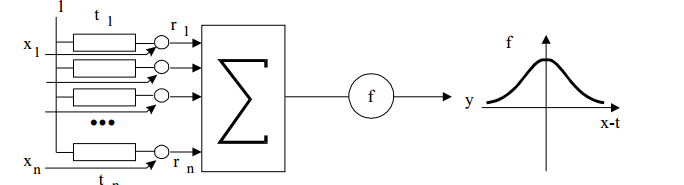
\includegraphics[scale=0.6]{radial}
\end{figure}

Neuron radialny - Agregacja sygnałów wejściowych
w tym typie neuronu polega na 
obliczaniu odległości pomiędzy 
obecnym wektorem wejściowym X
a ustalonym podczas uczenia 
centroidem pewnego podzbioru T.

Również nieliniowa funkcja 
przejścia w tych neuronach ma 
odmienną formę - „dzwonu” 
gaussoidy - czyli jest funkcją
niemonotoniczną.

Sieć typu RBF 
w zastosowaniu 
do klasyfikacji 
(wykrywa
i sygnalizuje 
skupiska 
danych 
wejściowych)

\paragraph{Neuron radialny} jest zdefiniowany przez swoje centrum i parametr - promień.
Obliczana jest odległość wektora wag i wektora sygnałów. Promień jest przechowywany
w neuronie jako wartość progowa.

\paragraph{Powtórne próbkowanie} Metoda ta polega na tym, że wybrane w sposób 
losowy elementy ze zbioru uczącego kopiowane są do neuronów radialnych 
(jako występujące w tych neuronach zestawy wag). Ponieważ podlegające 
kopiowaniu sygnały wejściowe wybrane zostały w sposób losowy, więc 
"reprezentują" one (w sensie statystycznym) rozkład wszystkich danych 
uczących. Jednakże, jeśli liczba neuronów radialnych nie jest duża, to neurony 
te mogą stanowić w rzeczywistości złą reprezentację (Haykin, 1994).

\paragraph{ k-średnich} Algorytm ten (Bishop, 1995) próbuje ustalić optymalny 
zbiór punktów, które stanowić będą centra skupień występujących w danych 
uczących. Mając K neuronów radialnych musimy wytworzyć K niezależnych 
centrów, w taki sposób, by reprezentowały one charakterystyczne skupiska 
wejściowych danych. Centra te ustala się w procesie iteracyjnym, w którym 
powtarzane są następujące czynności
\begin{enumerate}
 \item Każdy element zbioru uczącego przypisywany jest do tego centrum 
skupienia, które położone jest bliżej danego elementu niż wszystkie pozostałe 
centra
 \item Każde centrum skupienia wyznaczane jest jako wektor średnich wartości 
zmiennych wyznaczony dla wszystkich punktów należących do danego 
skupienia
\end{enumerate}
 
 \paragraph{Wybór promienia (odchylenia)}
 
 Definiowanie przez użytkownika. Użytkownik samodzielnie określa wielkość
odchylenia.
Równomierny przydział odchyleń. Odchylenie (identyczne dla wszystkich 
neuronów) jest określane za pomocą pewnej reguły heurystycznej, 
uwzględniającej liczbę centrów oraz wielkość zajmowanej przez nie 
przestrzeni (Haykin, 1994).
Przydział metodą k-najbliższych sąsiadów. Odchylenie dla każdego 
neuronu jest określane indywidualnie jako średnia odległość do jego k 
najbliższych sąsiadów (przypadków ze zbioru danych). Stąd odchylenia są
mniejsze w mocno zagęszczonym obszarze danych, co umożliwia zachowanie 
drobnych szczegółów i większe w obszarze, w którym dane występują rzadko 
(umożliwia to lepszą interpolację).

Zastosowanie RBF (zamiast MLP) 
spowoduje, że sieć neuronowa znajdzie 
aproksymację lepiej dopasowaną do 
lokalnych właściwości zbioru danych, 
ale gorzej ekstrapolującą.
\textbf{Sieci RBF bywają nadmiernie wrażliwe 
na nawet nieliczne błędy w danych 
uczących}

\paragraph{Sieć RBF} Ma ona strukturę dwuwarstwową, warstwa ukryta realizuje odwzorowanie 
nieliniowe realizowane przez neurony radialnej funkcji bazowej. 
Neuron wyjściowy jest liniowy, a jego rolą jest sumowanie wagowe 
sygnałów pochodzących od neuronów warstwy ukrytej.

\paragraph{Sieć radialna, a sieć sigmoidalna}

Sieci neuronowe o radialnych funkcjach bazowych znalazły zastosowanie
zarówno w rozwiązywaniu problemów klasyfikacyjnych, zadaniach
aproksymacji funkcji wielu zmiennych, jak i zagadnieniach predykcji tych
obszarach zastosowań gdzie funkcje sigmoidalne mają ugruntowaną pozycję.
W stosunku do sieci wielowarstwowych o sigmoidalnych funkcjach aktywacji
wyróżniają się pewnymi właściwościami szczególnymi, umożliwiającymi
lepsze odwzorowanie cech charakterystycznych modelowanego procesu.

\paragraph{funkcje radialne}

Sieci typu radialnego stanowią naturalne uzupełnienie sieci sigmoidalnych. 
Neuron sigmoidalny reprezentował w przestrzeni wielowymiarowej 
hiperplaszczyznę separującą tą przestrzeń na dwie kategorie (klasy), w 
których był spełniony odpowiedni warunek, albo 
$W_{ij} x_j > 0$ albo $W_{ij} x_j < 0$. 
Neuron radialny z kolei reprezentuje hipersferę, dokonującą podziału 
kołowego wokół punktu centralnego. 

\paragraph{Sieć radialna a sieć sigmoidalna}
\textbf{Sieć sigmoidalna}
Działanie funkcji rozciąga się od określonego punktu w przestrzeni aż do 
nieskończoności, reprezentuje aproksymację globalną funkcji zadanej. Nie 
ma niemożności fizycznego powiązania obszaru aktywności neuronu z 
odpowiednim obszarem danych uczących, trudności z określeniem 
optymalnego punktu startowego z procesie uczenia.
\textbf{Sieć radialna}
Bazuje na funkcjach mających wartość niezerową jedynie w określonej 
przestrzeni tylko wokół centrów, realizuje aproksymację typu lokalnego, 
której zasięg działania jest bardzo ograniczony. Można się spodziewać że 
zdolności do uogólniania są gorsze niż dla sieci sigmoidalnych. Łatwość
powiązania parametrów funkcji bazowych z fizycznym rozmieszczeniem 
danych w obszarze parametrów. Łatwość uzyskania dobrych wartości 
startowych w procesie uczenia pod nadzorem.

Przestrzenie decyzyjne tworzone w sieciach radialnych są stosunkowo 
proste i w sposób naturalny kształtowane. Sieć dostarcza nie tylko 
informacji do jakiej klasy należy wzorzec testujący, ale wskazuje również
na ewentualną możliwość utworzenia oddzielnej klasy. 
Na ogół uważa się, że sieci radialne lepiej niż sieci sigmoidalne nadają się
do takich żądań klasyfikacyjnych jak wykrywanie uszkodzeń w różnego 
rodzaju systemach, rozpoznawanie wzorców, itp. 
Znaczną zaletą sieci radialnych jest znacznie uproszczony algorytm 
uczenia. Przy istnieniu tylko jednej warstwy ukrytej i ścisłym powiązaniu 
aktywności neuronu z odpowiednim obszarem przestrzeni danych 
uczących, punkt startowy uczenia jest znacznie bliżej rozwiązania 
optymalnego, niż jest to możliwe w sieciach wielowarstwowych.

Dodatkowo, możliwe jest odseparowanie etapu doboru parametrów funkcji 
bazowych od doboru wartości wag sieci (algorytm hybrydowy), co może 
przyśpieszyć i uprościć proces uczenia. Przy zastosowaniu ortogonalizacji 
proces optymalnego kształtowania struktury sieci jest stałym fragmentem 
uczenia, nie wymagającym żadnego dodatkowego wysiłku. 
Liczba neuronów ukrytych decyduje w dużym stopniu o dokładności 
odwzorowania i zdolnościach uogólniania sieci. W przypadku sieci 
radialnej problem doboru liczby neuronów ukrytych jest o wiele prostszy 
niż w sieciach sigmoidalnych, ze względu na lokalny charakter 
aproksymacji reprezentowany przez poszczególne funkcje bazowe. 

Sieć RBF może być na różne sposoby hybrydyzowana -
może być na przykład uczona algorytmem Kohonena i LVQ, co jest 
alternatywą do przypisywania centrów odzwierciedlającego rozkład 
danych. Warstwa wyjściowa (liniowa lub nie) może być uczona 
którymkolwiek z iteracyjnych algorytmów dla warstw z iloczynem 
skalarnym.

\paragraph{Dobór parametrów funkcji radialnych}

Znacznie lepsze rezultaty można uzyskać przez zastosowanie 
samoorganizujacego się procesu podziału danych uczących
na klastry w jednej z jego licznych odmian. 
Centrum klastra jest utożsamiane z centrum odpowiedniej funkcji radialnej. 
Liczba tych funkcji jest równa liczbie klastrów i może być korygowana przez 
algorytm samoorganizacji. 
Proces podziału danych na klastry może być przeprowadzany metodą
K-uśrednień. Aparat matematyczny zaangażowany w tą procedurę jest dość
skomplikowany.

\paragraph{Sieć klasy GRNN}

Warstwa wejściowa, radialna, regresyjna oraz wyjściowa.
\begin{enumerate}
 \item Wejściowe wektory uczące dzielone są na 
skupienia - w szczególnym przypadku każdy 
wektor tworzy oddzielne skupienie
 \item Dla każdego skupienia znana jest wartość
zmiennej objaśnianej (wyjście sieci)
 \item wartość zmiennej objaśnianej dla dowolnego 
wektora wejściowego szacowana jest jako 
średnia ważona liczona z wartości tej 
zmiennej dla skupień - wagi uzależnione są
od odległości wejścia od centrów skupień
\end{enumerate}
\section{Wykład 8 - sieci rezonansowe}

Wagi w dół - pamięć krótkotrwała
Wagi w górę - pamięć długotrwała

\url{http://iisi.pcz.pl/nn/rezonnsowe.php?art=5}

Głównym powodem dla którego w tym wykładzie nic nie ma jest przekroczenie poziomu chujowości wykładu ponad mój już i tak
bardzo tolerancyjny próg. W związku z tym, że sieci rezonansowe w linku są ładnie opisane odsyłam do powyższego.
\section{Wykład 9 - sieci rekurencyjne}

\paragraph{Sprzężenie zwrotne w neuronie liniowym}

Po jednorazowym impulsie na wejściu na wyjściu otrzymamy długotrwały proces, w którym sygnał wyjściowy zmienia
się wielokrotnie, aż osiągnie stan równowagi (jeśli go osiągnie).
Równowaga w sieci może być osiągnięta (bez
działającego sygnału wejściowego) jedynie w taki
sposób, że sygnał wyjściowy po przemnożeniu przez
wagę sprzężenia zwrotnego daje taki sam sygnał. Taki
sygnał nazywamy ATRAKTOREM. Położenie
atraktora jest związane z parametrami sieci. Dla
współczynnika wagowego sprzężenia zwrotnego o
wadze 1 każdy punkt jest atraktorem, natomiast dla
dowolnej sieci stan równowagi uzyskujemy tylko
wtedy, gdy sygnał wyjściowy ma wartość 0.

Jeśli wartość współczynnika wagi synaptycznej w obwodzie sprzężenia zwrotnego jest dodatnia
to przebiegi mają charakter aperiodyczny (nie mają oscylacji). Wartości nie zmieniają znaku oraz 
są monotoniczne (rosną dla dodatnich, maleją dla ujemnych).

Jeśli wartości współczynnika wagi synaptycznej są ujemne to system ma charakter periodyczny.

Istnieje pojęcie niestabilności sieci. Jeśli sieci są stabilne to dążą do stanu równowagi.

Wartość sygnału wejściowego może być podawana cały czas.

\paragraph{Wnioski}

Przebieg sygnałów wyjściowych w sieci ze sprzężeniem zwrotnym może wykazywać dwojakiego rodzaju
zmienność. W przypadku nieliniowego neuronu możliwe byłyby formy zachowania systemu char. dla
systemów nielinowych to jest chaotyczne błądzenie \textit{ze wszystkimi cudeńkami współczestnej
teorii chaosu - efekt motyka, dziwne atraktory, fraktale, zbiory Mandelbrotta}.

\paragraph{Trzy warunki stabilności sieci Hopfielda}

\begin{enumerate}
 \item wprowadzono bardzo regularną strukturę wewnętrzną sieci - neurony są łączone każdy z każdym
 
 \item zabroniono sprzężeń zwrotnych obejmujących jeden neuron
 
 \item wprowadzone współczynniki wagowe muszą być symetryczne - jak $x$ do $y$ ma wagę $w$ to $y$ do $x$ ma wagę $w$
 
\end{enumerate}

Istnieje pojęcie funkcji energetycznej dla sieci Hopfielda. Wynika z niej, że zmiana y ma znak identyczny
ze znakiem łącznego pobudzenia. Zmiana energii podczas aktualizacji wyjść jest zawsze niedodatnia.

\paragraph{METODY WYKORZYSTUJĄCE JEDNOKROTNĄ PREZENTACJĘ WZORCÓW}

Metoda Hebba

\begin{equation}
 t_{ij}^s = \begin{cases}
    0,& \text{if} i = j \\
    \frac{1}{N} \sum_{s=1}^M x_i^s x_j^s & \text{otherwise} 
\end{cases}
\end{equation}

\begin{enumerate}
 \item $N$ - liczba bitów w obrazie wzorcowym
 \item $M$ - liczba wektorów wzorcowych
 \item $t_{ji}^s$ waga połączenia wyjścia j-tego neuronu z wejściem i-tego neuronu przy prezentacji s-tego obrazu wzorcowego
\end{enumerate}

Istnieję wersje metody hebba dla macierzy, wzorców unipolarnych oraz wersja iteracyjna.

Metoda wzajemnych ograniczeń - reguła Hebba ze składnikiem $\lambda$ \textit{odpychającym}

\begin{equation}
 t_{ij}^s = \begin{cases}
    0,& \text{if} i \ne j \\
    \sum_{s=1}^M x_i^s x_j^s - \lambda \sum_{p \ne s}^M x_i^p x_j^s & \text{otherwise} 
\end{cases}
\end{equation}

Istnieje również reguła rzutowania $\Delta$ oraz zmodyfikowana reguła perceptronu.
Zmodyfikowana reguła perceptronu różni się od hebba, że w procesie uczenia dodano składnik
bieżącej korekty błędów.

\paragraph{SIEĆ HOPFIELDA JAKO PAMIĘĆ SKOJARZENIOWA}

Tego typu sieci mogą 
działać jako pamięć 
autoasocjacyjna, czyli 
rozpoznają wzorce, 
którymi były uczone.
Wykorzystanie takiej pamięci
polega na tym, że potrafi ona
odtworzyć obraz na podstawie
obrazu silnie zniekształconego
lub zakłóconego.

\paragraph{Ciekawostka}

Rozwiązywanie problemu TSP przy wykorzystaniu
sieci Hopfielda jest mało efektywne. Nie istnieją
reguły dopasowania parametrów sieci a ich dobór
jest czasochłonny.
\end{document}